\documentclass[a4paper,12pt]{article}

\usepackage{tocloft}
\usepackage{algorithmic}
\usepackage{algorithm}

\setlength{\cftbeforesecskip}{0.2cm}
% Enter the inputs below
%-------------------------------------------------------------------------------
\newcommand{\studentName}{David Korčák}
\newcommand{\projectTitle}{GPU-based simulation and reinforcement learning pipeline for tracked ground robots}
\newcommand{\academicYear}{Prague, January 2025}
\newcommand{\docType}{B4BPROJ6 report}
\newcommand{\studyProgramme}{Open Informatics}
\newcommand{\branchOfStudy}{Artificial Intelligence and Computer Science}
\newcommand{\supervisorName}{doc. Ing. Karel Zimmermann, Ph.D.}
%-------------------------------------------------------------------------------

% Style file (.sty) with dissertation format
\usepackage{report_template}


\begin{document}


% TITLE AND DECLARATION PAGESFluids_MSc_DissertationFluids_MSc_Dissertation
%------------------------------------------------------------------------
\frontMatter
%------------------------------------------------------------------------


% ABSTRACT
%------------------------------------------------------------------------
\section*{Abbreviations}
\label{sec:abbreviations}
\addcontentsline{toc}{section}{Abbreviations}

\textbf{MPC} - Model Predictive Control \\ 
\textbf{RL} - Reinforcement Learning
%------------------------------------------------------------------------


\clearpage
\pagestyle{fancy}


% TABLE OF CONTENTS
%------------------------------------------------------------------------
% \vspace*{-2cm} % adjust the spacing as needed
\tableofcontents % Use \thispagestyle for correct headers and footers
%------------------------------------------------------------------------


\clearpage

% INTRODUCTION
%------------------------------------------------------------------------
\section{Introduction}
\label{sec:introduction}

In many robotics applications, simulation is a key component of development, testing, and in some particular cases, the deployment. Control and planning algorithms benefit greatly from high simulation accuracy, however, the computational cost of such simulations can be prohibitive. Certain methods requiring high number of time steps or large sample sizes can become infeasible to run and quickly iterate over. 

Two such areas are Model Predictive Control (MPC) and Reinforcement Learning (RL). MPC performs optimization over a finite horizon, requiring multiple simulation rollouts to find the optimal control sequence. RL, on the other hand, requires a large number of samples to learn the optimal policy. Both of these methods are known for leading to state-of-the-art results. In particular, they can solve complex, high-DoF control problems with relatively little manual engieering or tuning, mostly through an appropriate penalty (reward) function. Therefore, it makes sense to investigate and optimize the simulation pipeline to make these methods more accessible and more widely applicable.

The aim of this project is to enable the use of these methods on tracked robots used by the Vision for Robotics and Autonomous Systems group by developing a GPU-based simulation pipeline, capable of running multiple times faster than real-time. The underlying simulation engine will be based on formulation proposed by \citet{Agishev_2024}. The engine will be integrated into a PyTorch-native \citep{paszke2019pytorchimperativestylehighperformance} simulation and reinforcement learning toolkit based on TorchRL \citep{bou2023torchrldatadrivendecisionmakinglibrary}. The pipeline will be evaluated on throughput (performance scaling with respect to the number of robots simulated at once) and numerical stability over time.





\clearpage


% BACKGROUND
%------------------------------------------------------------------------
\section{Background}
\label{sec:background}

This should consist of a relevant background to the subject. This will involve a literature survey, which need not be exhaustive but should be critical and concentrate on the most relevant, (possibly controversial aspects) to the work described in the report. It should not occupy a large part of the dissertation, unless it in some way forms the core of the work. The primary objective of the literature review is to establish the ‘state-of-science’ and to demonstrate, through critique of existing work, why the approaches to be outlined subsequently are worth pursuing.

\textbf{All equations must be numbered}. For example here is the 2D mass continuity equation for incompressible fluids


\begin{equation}
  \label{eq:mass-continuity}
  \frac{\partial u}{\partial x} + \frac{\partial w}{\partial z} = 0
\end{equation}

and here is the equation for irrotational 2D flows

\begin{equation}
  \label{eq:irrotationality}
  \frac{\partial w}{\partial x} - \frac{\partial u}{\partial z} = 0
\end{equation}
%------------------------------------------------------------------------


\clearpage


\section{Simulation of tracked robots}
\label{sec:robots_props}

\subsection{Tracked robots}
\label{sec:robots}

The Vision for Robotics and Autonomous Systems group utilises 2 kinds of tracked robots, each with a different propulsion setup. The first robot is \textbf{MARV} (Mobile Advanced Robotic Vehicle), developed by \href{https://jettyvision.cz/servisni-robot-marv/}{JettyVision}. It is a battery-powered robot with 4 independent tracks, each driven by a separate motor. Each of the tracks is capable of rotating around its main motor axis on a 180-degree arc, allowing the robot to conform to uneven terrain. In the rest of the report, these rotating tracks will be referred to as \textit{flippers}.

\begin{figure}[!h]
  \centering
  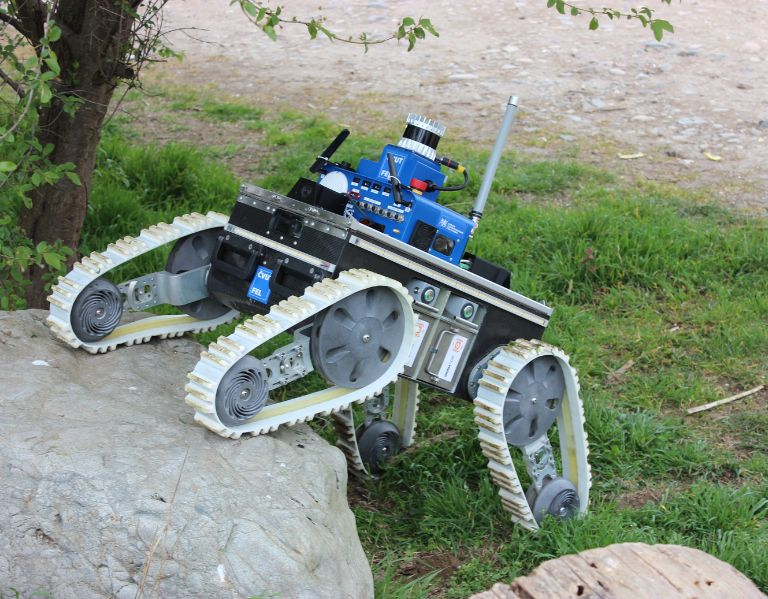
\includegraphics[width=0.4\textwidth]{fig/marv.jpg}
  \caption{MARV robot}
  \label{fig:marv}
\end{figure}

The second robot, codenamed \textbf{TRADR}, was developed within the \href{https://www.tradr-project.eu/}{TRADR project}. Designed as a disaster-response robot, it is equipped with a more elaborate traction setup than \textit{MARV}. It features 4 flippers and adds a wide, fixed track along the robot's entire length on each side. The flippers share their rotation axes with the fixed track's wheels. 

\begin{figure}[!h]
  \centering
  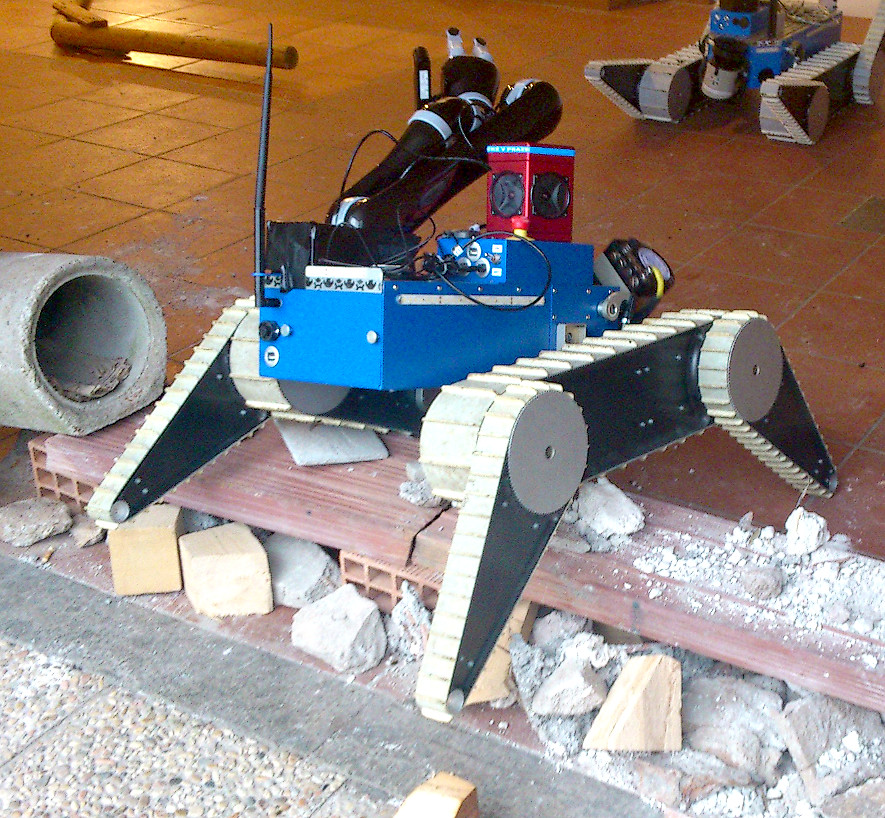
\includegraphics[width=0.4\textwidth]{fig/tradr.jpg}
  \caption{TRADR robot}
  \label{fig:tradr}
\end{figure}

Both robots can reach speeds of up to 1 m/s and are capable of off-road operation.

\clearpage

\subsection{Robot modeling}
\label{sec:modeling}
\subsubsection{Simplification of robot geometry}
For each of the robots, high-resolution triangular meshes are available. However, they are highly detailed and contain many unnecessary vertices, especially in details such as the cameras, LiDAR, or other small components. Because these parts of the robot never come into contact with the environment, they can be removed. Further details such as battery trays are not relevant either. This allows for a significant reduction in the number of vertices in the irrelevant parts of the robot. Overall, the most crucial component for collision detection and contact force computation is the flipper itself. Therefore, an elaborate process of simplifying the flippers' geometry and extracting their surface is used, while the rest of the robot is simplified by voxelization of a delaunay-triangulated envelope. The entire process of simplifying the robot geometry is shown in Algorithm~\ref{alg:mesh_simplification}.

\begin{algorithm}[H]
  \caption{Simplification of Robot Geometry  - see \href{https://github.com/edavidk7/tracked_sim_rl/blob/main/configs/robot_config.py\#L143}{code}}
  \label{alg:mesh_simplification}
  \begin{algorithmic}
    \vspace{0.25cm}
    \STATE \textbf{Procedure} ExtractSurfaceFromMesh(\textit{mesh}, \textit{n\_points}, \textit{clus\_opts})
        \STATE Perform Delaunay 3D triangulation on \textit{mesh}
        \STATE Extract the surface geometry
        \STATE Cluster surface points to \textit{n\_points}
        \RETURN Clustered centroids as \textit{Tensor}
    \vspace{0.25cm}

    \STATE \textbf{Procedure} SimplifyDrivingPart(\textit{mesh}, \textit{n\_points}, \textit{clus\_opts}, \textit{voxel\_size})
        \STATE Subsample points using ClusterPoints(\textit{mesh.points}, \textit{n\_points}, \textit{clus\_opts})
        \STATE Voxelize subsampled mesh using VoxelizeMesh(\textit{mesh}, \textit{voxel\_size})
        \RETURN Simplified mesh for driving part
        \vspace{0.25cm}
    \STATE \textbf{Procedure} SimplifyRobotBody(\textit{mesh}, \textit{n\_points}, \textit{clus\_opts}, \textit{voxel\_size})
        \STATE Extract \textit{surface} from \textit{mesh} using Delaunay3D
        \STATE Voxelize surface using VoxelizeMesh(\textit{surface}, \textit{voxel\_size})
        \RETURN Voxel centroids 
      \vspace{0.25cm}
    \STATE \textbf{Procedure} SimplifyRobotGeometry(\textit{body\_mesh}, \textit{part\_meshes}, \textit{n\_points}, \textit{clus\_opts}, \textit{voxel\_size})

      \STATE Simplify the body mesh using SimplifyRobotBody(\textit{body\_mesh}, \textit{n\_points}, \textit{clus\_opts}, \textit{voxel\_size})

        \FOR{\textbf{each} \textit{part\_mesh} in \textit{part\_meshes}}
            \STATE Simplify \textit{part\_mesh} using SimplifyDrivingPart(\textit{part\_mesh}, \textit{n\_points}, \textit{clus\_opts}, \textit{voxel\_size})
        \ENDFOR
        \RETURN Simplified robot geometry
        \vspace{0.25cm}
    \end{algorithmic}
    
  \end{algorithm}


\clearpage

\begin{figure}
  \centering
  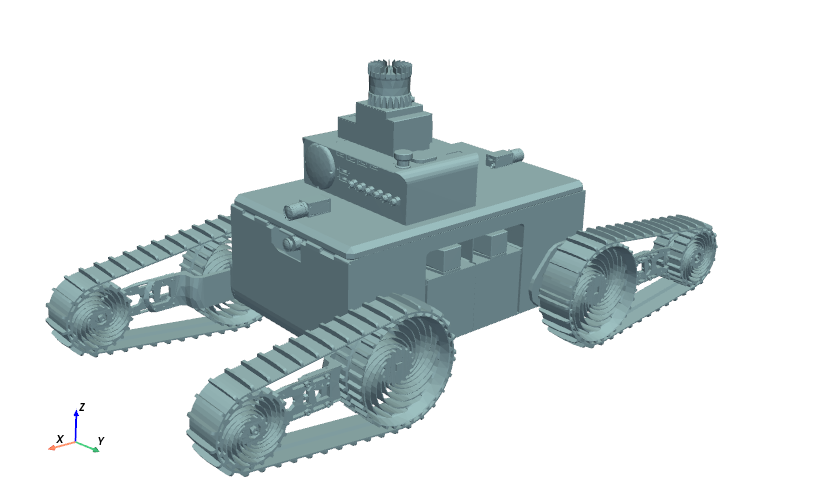
\includegraphics[width=0.6\textwidth]{fig/full_marv_mesh.png}
  \caption{Full MARV mesh}
  \label{fig:full_marv_mesh}
\end{figure}

\begin{figure}[H]
  \centering
  % row 1
  \begin{subfigure}[t]{0.45\textwidth}
      \centering
      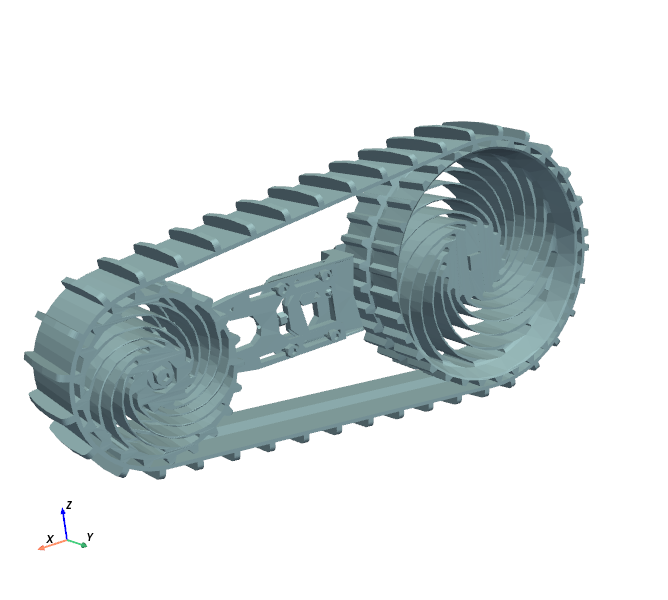
\includegraphics[width=\textwidth]{fig/full_flipper_mesh.png} % replace with your image path
      \caption{Full flipper mesh.}
      \label{fig:fig1}
  \end{subfigure}
  \hfill
  \begin{subfigure}[t]{0.45\textwidth}
      \centering
      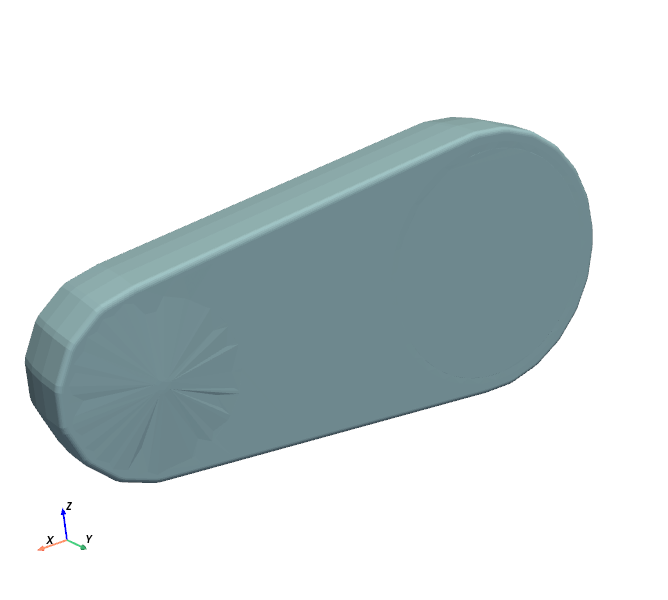
\includegraphics[width=\textwidth]{fig/flipper_delaunay.png} % replace with your image path
      \caption{3D Delaunay triangulation of the flipper mesh.}
      \label{fig:fig2}
  \end{subfigure}

  \vspace{0.5cm} % spacing between rows

  % row 2
  \begin{subfigure}[t]{0.45\textwidth}
      \centering
      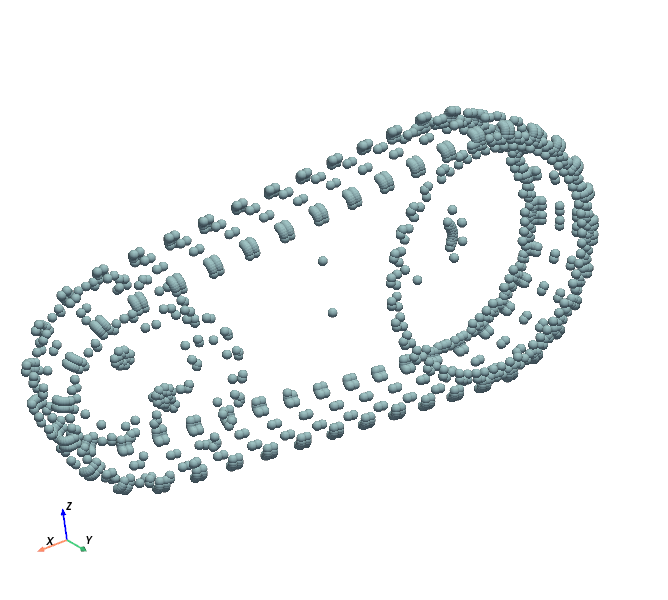
\includegraphics[width=\textwidth]{fig/flipper_surface_points.png} % replace with your image path
      \caption{Extracted surface points.}
      \label{fig:fig3}
  \end{subfigure}
  \hfill
  \begin{subfigure}[t]{0.45\textwidth}
      \centering
      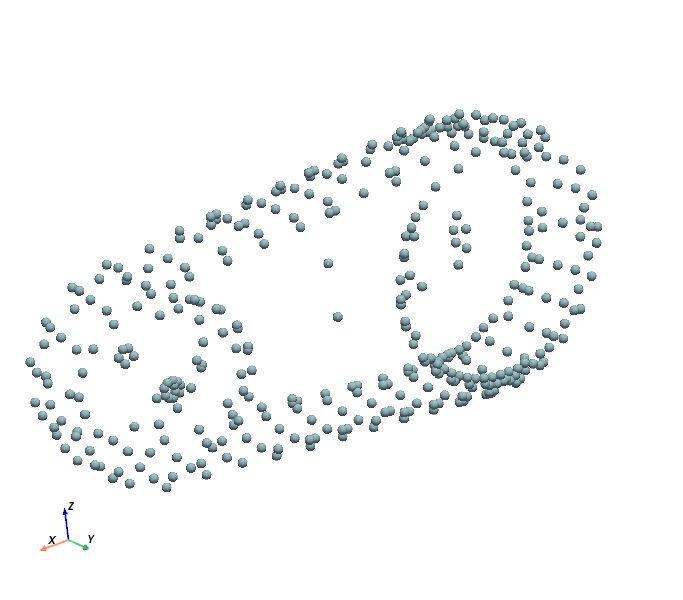
\includegraphics[width=\textwidth]{fig/flipper_clustered.png} % replace with your image paths
      \caption{Clustered surface points.}
      \label{fig:fig4}
  \end{subfigure}

  \caption{Simplification of the flipper geometry.}
  \label{fig:4figures}
\end{figure}

\clearpage

\subsubsection{Inertial properties} 
The robots' inertial properties are crucial for the simulation's accuracy, especially the force interactions. Here, we improve greatly over \citet{Agishev_2024}, where the robot's mass was distributed uniformly across the robot's points (globally simplified by voxelization). This is not realistic, as the robot's mass is concentrated in the robot's body (due to the presence of batteries, onboard computer, and sensors). Futher, the difference in point-per-unit-volume between the flippers and body parts of the mesh would lead to erroneous Center-of-Gravity placement and moment of inertia.

We address this with a simple modification. We model the discrepancy in volumetric density between the body and the flippers by assigning a lower relative mass to points in the flippers. The body's density is set to 1, while the flippers' density $\rho_\text{driving parts} \in \left(0.1,0.5\right)$. Using this modification, we distribute the mass of the robot in a pointwise fashion. Let $m$ be the total mass of the robot. Then, the mass of each point $i$ is given by Equation~\ref{eq:mass_distribution}, \href{https://github.com/edavidk7/tracked_sim_rl/blob/main/configs/robot_config.py\#L173}{code}.

\begin{equation}
  \label{eq:mass_distribution}
  m_i = \begin{cases}
    \frac{1}{Z} \cdot m & \text{if } i \in \text{body} \\
    \frac{\rho_\text{driving parts}}{Z} \cdot m & \text{if } i \in \text{driving parts}
  \end{cases} 
\end{equation}

where $Z = \sum_{i} \llbracket {i \in \text{body}} \rrbracket + \rho_\text{driving parts} \cdot \sum_{i} \llbracket {i \in \text{driving parts}} \rrbracket$ is the normalization constant. 

\subsubsection{Controls and kinematics}

To model the robot's propulsion, we relax the accuracy of the simulation and use a very simplified setup. The control velocity modeled by four scalar velocities, each corresponding to the speed of the track at the point of contact with the ground. Velocity vectors of each track are acting the robot's local x-coordinate, or its forward-facing direction (positive x). The robot's rotational velocity is generated by varying the speeds of the tracks between the left and right side. This is the simplest possible model of a tracked robot's kinematics, and it is part of our future work to improve it. As mentioned in Section \ref{sec:background}, none of the widely used simulation toolkits support tracked robots, as it is a very complex problem to solve, \href{https://github.com/edavidk7/tracked_sim_rl/blob/main/engine/engine.py#L147}{code}.

The control input for the flippers' articulation is a tuple of 4 scalar values, each representing the rotational velocity of the flipper around its y-axis, \href{https://github.com/edavidk7/tracked_sim_rl/blob/main/engine/engine.py#L92}{code}.

Overall, our control vector is $\mathbf{u} = \left(v_1, v_2, v_3, v_4, \omega_1, \omega_2, \omega_3, \omega_4\right)$, where $v_i$ is the velocity of the $i$-th track and $\omega_i$ is the rotational velocity of the $i$-th flipper.

\section{Physics simulation engine}
\label{sec:engine}


This should describe the general basis of the research approach – such as the form of hypotheses, general methods of statistical analysis, analytical framework, experimental procedures, numerical setup, etc... Your methodology needs to be adequately described and its use fully justified.
%------------------------------------------------------------------------


\clearpage


% RESULTS AND DISCUSSION
%------------------------------------------------------------------------
\section{Results and Discussion}
\label{sec:results-discussion}

Describe results in a logical order, which is not necessarily the order in which you performed the project. It is a common failing to assume that the reader knows the project as well as you do. He or she must not be expected to use the arts of a detective to find and decipher the important information. Therefore, refer appropriately to figures or tables and remember to emphasise and perhaps quote significant results. Do not deluge the reader with data and figures; use appendices for details if necessary and concentrate on key results in the body of the text. Briefly summarise the main results at the end of each main sequence of experiments/simulations.

Analysis of your results should include, for example, clear graphical representations, and, when necessary, appropriate statistical analysis.

The Discussion part should attempt to tie together the results and what they indicate in a broader
context, including discussion in relation to the literature and implications beyond the immediate
confines of your specific project. It should also illustrate the extent to which the original aims
have been satisfied, any difficulties you have identified and what future work is suggested.
\textbf{Great care is needed with this with this part of the dissertation.} 

\clearpage

Here is an example of how to use figures within the dissertation:

\begin{quote}
  Figure~\ref{fig:wave_breaking_lab_measurements} illustrates the breaker index as a function of the
  Irribarren number $N_I$, as found by the experimental investigations undertaken by
  \citet{Battjes1974}.
\end{quote}

\begin{figure}[!h]
  \centering
  
\includegraphics[width=0.6\textwidth]{ctu_lion.pdf}
  \caption{Breaker index, $\gamma$, versus Irribarren number, $N_I$, fit to experimental measurements \citep{Battjes1974}.}
  \label{fig:wave_breaking_lab_measurements}
\end{figure}

Here is an example of using tables within the dissertation:

\begin{quote}
  The wave conditions within the coastal zone are dependent on the water depth regime in which the
  waves propagate. Table~\ref{tab:water-depth-regimes} presents the values of the relative water
  depth and group velocity for each water depth regime.
\end{quote}

\begin{table}[!h] 
  \centering
    \begin{tabular}{| l | c | c |}
     \bf Regime              &  \bf Relative water depth           &  \bf Group velocity        \\
        \hline
         Deep water          &  $kd > 4$                       &  $c_g = 0.5c$  \\
         Intermediate water  &  $0.3\leqslant kd \leqslant 4$    &  $c_g=\frac{c}{2}\left( 1 + \frac{2kd}{\sinh{(2kd)}}\right)$  \\
         Shallow water       &  $kd < 0.3$                     &  $c_g = c$\\
    \end{tabular}
    \caption{The relative water depth, $kd$, and group velocity, $c_g$, in terms of the phase velocity, $c$, for the various water depth regimes.}
    \label{tab:water-depth-regimes}
\end{table}
%------------------------------------------------------------------------

\clearpage


% CONCLUSIONS
%------------------------------------------------------------------------
\section{Conclusions}
\label{sec:conclusions}


This chapter is important to summarise your overall conclusions. It should be brief, with the final
conclusions and/or recommendations clearly identifiable without having to search for them. The use
of bullet points might help if you have a large number of conclusions. It should not simply repeat
what has been discussed in the preceding sections, but should summarise. It should not contain new information. It should then draw wider conclusions, including implications beyond the immediate case study or survey. The effective drawing out of these wider conclusions is what often marks out an excellent dissertation from a good or average dissertation. How does your research fit in the context of the existing literature you will already have reviewed: is it consistent or contradictory; have you found out anything `new'? This is also where you should clearly state any recommendations for future research.

This section, however, is not the only place where conclusions can be drawn and presented.  Individual sections are likely to have their own summaries and conclusions that will lead into the more comprehensive discussion section and a final summary and conclusions section.
%------------------------------------------------------------------------


\clearpage

% Data, code and use of Generative AI tools (e.g. ChatGPT)
%------------------------------------------------------------------------
\section{Use of Third-party Data, Code and Generative AI Tools}
\label{sec:DCG_Usaage}

This section is where you are required to acknowledge and report the source of any third-party data and code used in your work. For example, you may have used data collected in a previous experiment (physical or numerical) and you may have used code written by others to process those data. In addition, if you have used Generative Artificial Intelligence tools (e.g. ChatGPT) in anyway you are required to state how you have used these tools.

This section does not count towards your 50-page upper limit.

\clearpage


% REFERENCES
%------------------------------------------------------------------------
\bibliographystyle{report_template}
\bibliography{references}
\addcontentsline{toc}{section}{References} %Add this to the contents page

\vspace*{10mm}

\textbf{You will be penalised for incorrect referencing in your final dissertation.} Cite all references, with the name of the author(s) and year of publication in brackets. More than
two authors are quoted as first author \textit{et al.} followed by the year.  Two or more publications within
the same year by the same authors should be distinguished by the letters a, b, c, etc... Collect all
references together at the end of the report and list them alphabetically in standard form; \textbf{an
example of this is given above.} The \textbf{Harvard system} should be used and examples of it’s use in the body of text are given below:


\begin{quote}
This procedure is widely used \citep{Christou2009,Wu2016,Hughes2016a,Hughes2016b}. \citet{Christou2014} state that.... \citet{Spinneken2009a,Spinneken2009b} concluded that...
\end{quote}


Please note that it is important to have consistency in the style you use throughout your dissertation. \textbf{List only the references you cite in the text.} Any references not seen in the original language should be marked with an asterisk (*). If only seen as a translation, follow references with ``English translation''. Websites should be referenced in the main body of the text as other references (by author or organisation), with the final reference list containing details of the full URL the authority or organisation concerned, and the date at which it was accessed (since websites may change and may not be able to be accessed subsequently). You should avoid relying too heavily on websites – try to reinforce your referencing with sufficient academic literature. Journals accessed electronically are still journals and quoted as normal.
%------------------------------------------------------------------------


\clearpage


% APPENDICES
%------------------------------------------------------------------------
\appendix

\section{Appendix Title}
\label{sec:appendix}

Label your appendices alphabetically: A, B, C, etc... using the Heading Appendix style. Add as many as you require, however please make sure that their content is relevant to report and not just a dump of every single thing that you did during your project. You may be penalised if the Appendix is excessive and not relevant, e.g. if appendices appear unconnected with the main text.

\textbf{Under no circumstances should important material be included in the Appendix, instead of the
  main text, in order to stay within the word limit.}

Large sets of relevant data (e.g., census results, "raw" experimental results) should be presented in an Appendix. Any useful parts of the study not directly relevant to the main theme may also be put in an Appendix, but should be clearly referenced in the text. 

Computer programs: if the program has been published, give a reference to it and a brief outline of the methods it uses. If the program is original give a listing as an Appendix preceded by a single page description of the program or on a data stick, as recommended by your supervisor.
%------------------------------------------------------------------------


\end{document}



